\documentclass[tikz, border=10pt]{standalone}
\usepackage{amssymb}
\usepackage{amsmath}
\usetikzlibrary{calc, positioning}

% Macro para célula vazia
\newcommand{\blankcell}{\phantom{a_{00}}}

% --- Layers ---
\pgfdeclarelayer{bg}
\pgfdeclarelayer{fg}
\pgfsetlayers{bg,main,fg}

\begin{document}

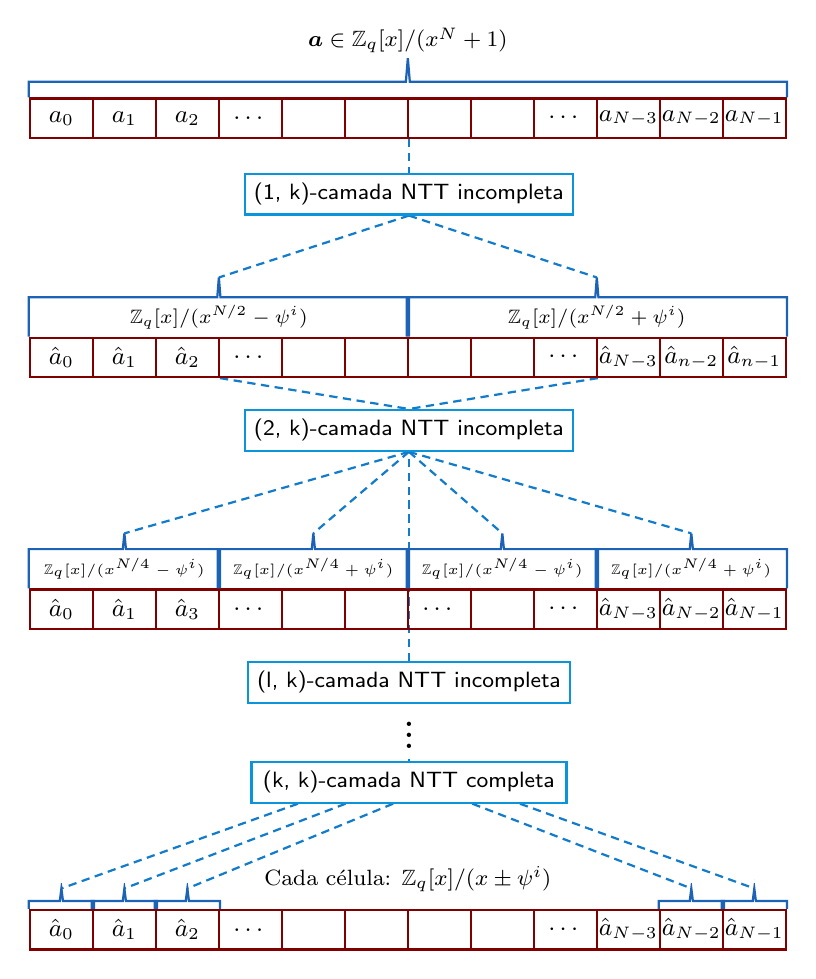
\begin{tikzpicture}[
    font=\small,
    arraybox/.style={
        draw=red!50!black,
        thick,
        minimum width=0.8cm,
        minimum height=0.5cm,
        inner sep=0pt,
        anchor=west
    },
    processbox/.style={
        draw=cyan!80!blue,
        thick,
        fill=white,
        rectangle,
        minimum height=0.35cm,
        minimum width=4cm,
        align=center,
        font=\sffamily\footnotesize
    },
    braceLine/.style={
        thick,
        draw=cyan!40!blue
    },
    connector/.style={
        densely dashed,
        thick,
        draw=cyan!60!blue
    },
    braceLbl/.style={
        align=center,
        inner sep=0pt,
        fill=white,
        fill opacity=0.95,
        text opacity=1,
        font=\scriptsize
    }
]

% =========================================================
% STRAIGHT BRACE
% =========================================================
% #4 = H (Altura vertical da perna/gap)
% #5 = Notch Height (Altura do bico triangular)
% #6 = W (Largura da base do bico) -> DIMINUIR ISSO AFINA A PONTA
\newcommand{\StraightBraceNamed}[9]{%
  \pgfmathsetmacro{\SBhalfW}{0.5*(#6)}%

  \path let \p1=(#2.north west), \p2=(#3.north east) in
    coordinate (#1-L)     at (\x1,\y1)
    coordinate (#1-R)     at (\x2,\y2)
    coordinate (#1-mid)   at ($(\x1,\y1)!0.5!(\x2,\y2)$)
    coordinate (#1-topL)  at ($(\x1,\y1)+(0,#4)$)
    coordinate (#1-topR)  at ($(\x2,\y2)+(0,#4)$)
    coordinate (#1-notchL) at ($(#1-mid)+(-\SBhalfW,#4)$)
    coordinate (#1-notchR) at ($(#1-mid)+(\SBhalfW,#4)$)
    coordinate (#1-notch)  at ($(#1-mid)+(0,{#4 + #5})$);

  \draw[braceLine]
    (#1-L) -- (#1-topL) -- (#1-notchL) -- (#1-notch) -- (#1-notchR) -- (#1-topR) -- (#1-R);

  \begin{pgfonlayer}{fg}
    \def\pos{#7}%
    \def\inside{inside}%
    \ifx\pos\inside
      % Texto no meio da perna
      \node[braceLbl, font=#8, anchor=center] (#1-lbl) at ($(#1-mid)+(0,{#4*0.5})$) {#9};
    \else
      \node[braceLbl, font=#8, anchor=south] (#1-lbl) at ($(#1-notch)+(0,0.06)$) {#9};
    \fi
  \end{pgfonlayer}
}

\def\cellw{0.8}

% ==========================================
% NÍVEL 0
% ==========================================
\foreach \i/\val in {
    0/a_0, 1/a_1, 2/a_2, 3/\dots,
    4/\blankcell, 5/\blankcell, 6/\blankcell, 7/\blankcell, 8/\cdots,
    9/a_{N-3}, 10/a_{N-2}, 11/a_{N-1}
} {
    \node[arraybox] (n0_\i) at (\i*\cellw, 0) {$\val$};
}

% Topo: #6 reduzido para 0.05
\StraightBraceNamed{B0}{n0_0}{n0_11}{0.20}{0.30}{0.05}{above}{\footnotesize}
{$\boldsymbol{a}\in\mathbb{Z}_q[x]/(x^N+1)$}

% ==========================================
% PROCESSO 1
% ==========================================
\node[processbox] (proc1) at ($(n0_5.south east) + (0, -0.7)$) {(1, k)-camada NTT incompleta};

\begin{pgfonlayer}{bg}
  \draw[connector] ($(n0_5.south east)$) -- (proc1.north);
\end{pgfonlayer}

% ==========================================
% NÍVEL 1
% ==========================================
\coordinate (row1_y) at ($(proc1.south) + (0, -1.8)$);

\foreach \i/\val in {
    0/\hat{a}_0, 1/\hat{a}_1, 2/\hat{a}_2, 3/\dots,
    4/\blankcell, 5/\blankcell, 6/\blankcell, 7/\blankcell, 8/\cdots,
    9/\hat{a}_{N-3}, 10/\hat{a}_{n-2}, 11/\hat{a}_{n-1}
} {
    \node[arraybox] (n1_\i) at ($(0,0 |- row1_y) + (\i*\cellw, 0.)$) {$\val$};
}

% #6 (largura do bico) reduzido de 0.40 para 0.04 (bem fino)
\StraightBraceNamed{B1L}{n1_0}{n1_5}{0.50}{0.25}{0.04}{inside}{\scriptsize}
{$\mathbb{Z}_q[x]/(x^{N/2}-\psi^i)$}

\StraightBraceNamed{B1R}{n1_6}{n1_11}{0.50}{0.25}{0.04}{inside}{\scriptsize}
{$\mathbb{Z}_q[x]/(x^{N/2}+\psi^i)$}

\begin{pgfonlayer}{bg}
  \draw[connector] (proc1.south) -- (B1L-notch);
  \draw[connector] (proc1.south) -- (B1R-notch);
\end{pgfonlayer}

% ==========================================
% PROCESSO 2
% ==========================================
\node[processbox] (proc2) at ($(proc1) + (0, -3.0)$) {(2, k)-camada NTT incompleta};

\begin{pgfonlayer}{bg}
  \draw[connector] ($(n1_2.south east)$) -- (proc2.north);
  \draw[connector] ($(n1_8.south east)$) -- (proc2.north);
\end{pgfonlayer}

% ==========================================
% NÍVEL 2
% ==========================================
\coordinate (row2_y) at ($(proc2.south) + (0, -2.0)$);

\foreach \i/\val in {0/\hat{a}_0, 1/\hat{a}_1, 2/\hat{a}_{3}} {
  \node[arraybox] (n2A_\i) at ($(n1_0.west |- row2_y) + (\i*\cellw, 0)$) {$\val$};
}
\foreach \i/\val in {0/\dots, 1/\blankcell, 2/\blankcell} {
  \node[arraybox] (n2B_\i) at ($(n1_3.west |- row2_y) + (\i*\cellw, 0)$) {$\val$};
}
\foreach \i/\val in {0/\dots, 1/\blankcell, 2/\cdots} {
  \node[arraybox] (n2C_\i) at ($(n1_6.west |- row2_y) + (\i*\cellw, 0)$) {$\val$};
}
\foreach \i/\val in {0/\hat{a}_{N-3}, 1/\hat{a}_{N-2}, 2/\hat{a}_{N-1}} {
  \node[arraybox] (n2D_\i) at ($(n1_9.west |- row2_y) + (\i*\cellw, 0)$) {$\val$};
}

% #6 reduzido de 0.30 para 0.04
\StraightBraceNamed{B2A}{n2A_0}{n2A_2}{0.50}{0.20}{0.04}{inside}{\tiny}
{$\mathbb{Z}_q[x]/(x^{N/4}-\psi^i)$}

\StraightBraceNamed{B2B}{n2B_0}{n2B_2}{0.50}{0.20}{0.04}{inside}{\tiny}
{$\mathbb{Z}_q[x]/(x^{N/4}+\psi^i)$}

\StraightBraceNamed{B2C}{n2C_0}{n2C_2}{0.50}{0.20}{0.04}{inside}{\tiny}
{$\mathbb{Z}_q[x]/(x^{N/4}-\psi^i)$}

\StraightBraceNamed{B2D}{n2D_0}{n2D_2}{0.50}{0.20}{0.04}{inside}{\tiny}
{$\mathbb{Z}_q[x]/(x^{N/4}+\psi^i)$}

\begin{pgfonlayer}{bg}
  \draw[connector] (proc2.south) -- (B2A-notch);
  \draw[connector] (proc2.south) -- (B2B-notch);
  \draw[connector] (proc2.south) -- (B2C-notch);
  \draw[connector] (proc2.south) -- (B2D-notch);
\end{pgfonlayer}

% ==========================================
% FIM
% ==========================================
\node[processbox] (procl) at ($(proc2) + (0, -3.2)$) {(l, k)-camada NTT incompleta};
\node[font=\bfseries] (dots) at ($(procl.south) + (0, -0.3)$) {$\vdots$};
\node[processbox] (prock) at ($(dots.south) + (0, -0.3)$) {(k, k)-camada NTT completa};

\begin{pgfonlayer}{bg}
  \draw[connector] (procl.north) -- (proc2.south);
  \draw[connector] (dots.north) -- (procl.south);
  \draw[connector] (prock.north) -- (dots.south);
\end{pgfonlayer}

% ==========================================
% ÚLTIMA LINHA
% ==========================================
\coordinate (row3_y) at ($(prock.south) + (0, -1.6)$);

\foreach \i/\val in {
    0/\hat{a}_0, 1/\hat{a}_1, 2/\hat{a}_2, 3/\dots,
    4/\blankcell, 5/\blankcell, 6/\blankcell, 7/\blankcell, 8/\cdots,
    9/\hat{a}_{N-3}, 10/\hat{a}_{N-2}, 11/\hat{a}_{N-1}
} {
    \node[arraybox] (n3_\i) at ($(0,0 |- row3_y) + (\i*\cellw, 0)$) {$\val$};
}

% #6 reduzido aqui também para 0.04
\foreach \i in {0,1,2,10,11} {
  \StraightBraceNamed{B3\i}{n3_\i}{n3_\i}{0.10}{0.16}{0.04}{ }{\tiny}{}
}

\coordinate (pkA) at ($(prock.south west)!0.15!(prock.south east)$);
\coordinate (pkB) at ($(prock.south west)!0.30!(prock.south east)$);
\coordinate (pkC) at ($(prock.south west)!0.45!(prock.south east)$);
\coordinate (pkD) at ($(prock.south west)!0.70!(prock.south east)$);
\coordinate (pkE) at ($(prock.south west)!0.85!(prock.south east)$);

\begin{pgfonlayer}{bg}
  \draw[connector] (pkA) -- (B30-notch);
  \draw[connector] (pkB) -- (B31-notch);
  \draw[connector] (pkC) -- (B32-notch);
  \draw[connector] (pkD) -- (B310-notch);
  \draw[connector] (pkE) -- (B311-notch);
\end{pgfonlayer}

\begin{pgfonlayer}{fg}
\node[above=4pt, font=\footnotesize, fill=white, inner sep=2pt] at
  ($(n3_5.north east)!0.5!(n3_6.north west)$)
  {Cada célula: $\mathbb{Z}_q[x]/(x \pm \psi^i)$};
\end{pgfonlayer}

\end{tikzpicture}

\end{document}